\chapter{Object Caching}

\label{sec:object-caching}

\subsection{Replica Placement}
\label{sec:replica-management}

Ziel des Object Caching ist es die Zugriffszeit auf Objekte für Client zu verringern. Deshalb macht es Sinn, dass Repliken vom Client initiiert werden. Die Alternative wäre dass der Server die Repliken initiiert. Werden die Replikas vom Client initiiert spricht man von Client Caches. Client Caches verbessern die Zugriffszeit der Clients auf die Daten.

In unserem RMIwithObjectCaching-System besitzt jeder Client einen lokalen Cache auf derselben Maschine. Der Cache ist nicht in der Grösse limitiert, da die Testcases keine Szenarien mit vielen Objekten vorsehen.

\subsection{Update Distribution}
\label{sec:update-distribution}

Werden Kopien von Objekten in einem lokalen Cache angelegt, müssen diese Kopien aktualisiert werden. Um dies zu realisieren gibt es mehrere Möglich\-keiten.

\subsubsection{Invalidation versus Data Transfer}
\label{sec:inval-vers-data}

\begin{description}
\item[Invalidation protocol] Bei einem Invalidation protocol werden nur Meldungen an die lokalen Caches gesendet, die dem Cache mitteilen, dass ein Objekt nicht mehr aktuell ist. Der Vorteil dieser Möglichkeit ist, das eine Invalidierungsmeldung nur beim ersten Write versendet werden muss. Ausserdem müssen keine Objektdaten übertragen werden. Das Verfahren spart also Bandbreite. Ein invalidation protocol macht ist sinnvoll, wenn das read-to-write-Verhältnis klein ist.
\item[Transfer Data] Der zweite Ansatz ist bei jedem Update die kompletten Daten eines Objektes an die lokalen Caches zu versenden. In diesem Fall kann der Client immer aus dem lokalen Cache lesen. Dieser Ansatz macht Sinn bei einem hohen read-to-write Verhältnis.
\end{description}

\subsubsection{Pull versus Push}
\label{sec:pull-versus-push}

Die Verantwortung, der Cache Aktualisierung kann entweder beim Server oder beim Client liegen. Man unterscheided zwischen push-based und pull-based Protokollen.

\begin{description}
\item[push-based] Der Server sendet dem Client Updates ohne, dass der Client diese anfordert. Der Server muss Buch darüber führen, in welchen Caches Kopien aller Objekte vorhanden sind.
\item[pull-based] Clients überprüfen bei jedem Zugriff, ob die Daten im Cache aktuell sind. Wenn nicht müssen die Daten neu angefordert werden. Das macht den Zugriff auf Daten langsamer. Dafür muss sich der Server nicht darum kümmern.
\end{description}

In unsererem Cache werden Aktualisierungen durch push-based updated realisiert, da wir die Zugriffzeit für die Clients erhöhen wollen und sich die Anzahl der Clients in Grenzen hält. Der Server kann sich merken, welcher Cache welche Objekte enthält.

In unserem System sind alle Objekte zentral auf dem Server abgespeichert. Das Objekt auf dem Server ist das Referenzobjekt. Alle Clients sollen die Updateoperationen in der Reihenfolge sehen, wie sie beim Server eintreffen. Ist jedem Objekt eine Maschine für die Koordination zugeordnet, nennt man das Protokol primary-based. Die Maschine, die das Objekt verwaltet nennt man primary. Ist der primary eine fixer Server werden alle Updateoperationen remote an diesen Server gesendet. In diesem Fall spricht man von Remote-Write Protocol. Die Concurrency Control bleibt dabei die selbe. Der inkrementiert die Version für jedes Objekt nachdem er die die Update Methode ausgeführt hat. Erhält vor dem Update Call einen Updates des Clients wird eine Exception geworfen.

\subsection{Implementierung Object Konsistenz Protokol}
\label{sec:impl-object-kons}

Der Prozess Kontostand erhöhen läuft wie folgt ab.

\begin{enumerate}
\item Client $C1$ ruft \verb+getBalance()+ auf.
\item RMI-Stub führt einen Lookup für das Objekt im Cache aus.
\item Ist das Objekt nicht Cache, fordert es der Cache beim Server an.
\item \verb+getBalance()+ wird auf auf dem Objekt ausgeführt. Der Wert wird an den Stub zurückgegeben und der Stub leitet ihn an den Client weiter.
\item \verb+setBalance()+ wird an den lokalen Cache weitergeleitet. Dieser enthält eine eigene Concurrency Control. Die überprüft, ob das Objekt sich seit dem letzen \verb+getBalance+ nicht verändert hat. Hat es sich verändert, wird eine Exception ausgelöst. Die Methode ändert den lokalen Cache nicht, weil zu diesem Zeitpunkt noch nicht klar ist, ob die Methode ausgeführt werden kann. Ein anderer Client könnte, das Objekt inzwischen verändert haben. Nur der Server kann entscheiden, ob die Methode ausgeführt werden kann.
\item Die \verb+setBalance()+-Methode invalidiert das Objekt. Der Wert im Cache kann noch nicht festgeschrieben werden, da noch nicht sicher ist, ob die Update Methode ausgeführt werden kann. Der Wert wird sich sicher ändern. Entweder aufgrund des lokalen \verb+setBalance()+-Aufruf oder weil ein anderer Client \verb+setBalance()+ aufgerufen hat. Solange das Objekt invalidiert ist, muss es bei einem \verb+getBalance()+-Aufruf neu beim Server angeforder werden. Damit verhindert man eine unnötige Exception.
\item Erhält ein Client Cache ein Update \verb+update()+
\end{enumerate}

\begin{description}
\item [setBalance] Das Object muss im Cache invalidiert werden. Mit ConcurrencyControl kann überprüft werden, ob mit einer alten Version gearbeitet wurde.
\end{description}

\subsubsection{Mögliche Aufrufszenarien}
\label{sec:mogl-aufr}

Im ersten Szenario treten keine Konsistenzprobleme auf. Laufen die Methodenaufrufe in dieser Reihenfolge ab, benötigt das System keine Concurrency Control.
\begin{enumerate}
\item Beim ersten \verb|getBalance()| fordert der Cache ein neues Objekt an und speichert es.
\item Beim zweiten \verb|getBalance()|  liegt das Objekt bereits im Cache und muss nicht nochmals vom Server angefordert werden.
\item Ruft der Client ein \verb|setBalance()| auf, wird dieser Aufruf direkt an der Server weitergeleitet. Der Aufruf blockiert, bis der Server eine Antwort sendet. Der Server sendet zuerst allen Clients das Update danach sendet er das ReturnValue des Methodenaufrufs. Die Update-Message wird also vor dem ReturnValue versendet. Im ClientCache wird das Update und das ReturnValue verarbeitet. Es kann nicht gesagt werden, ob der Cache bereits ein Update erfahren hat, wenn  \verb|setBalance()|  zurückkehrt.
\item Nachdem der ClientCache die Update Nachricht des Server verarbeitet hat, ruft der Client nochmals \verb|getBalance()| auf, erhält er den Kontostand des neuesten Objektes.
\end{enumerate}

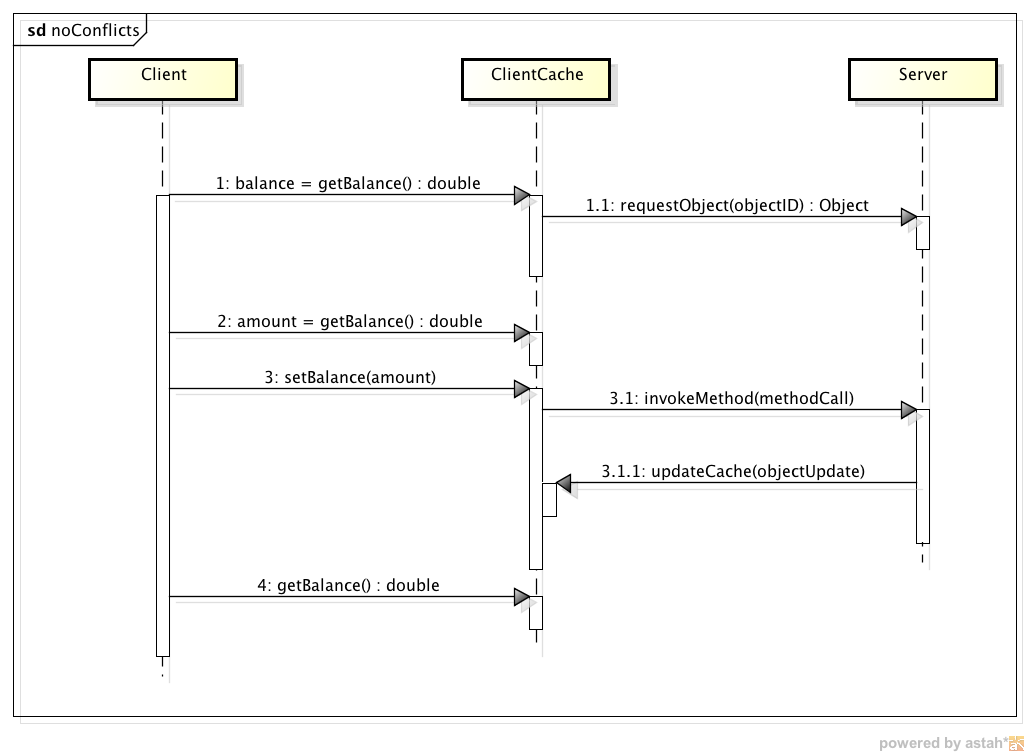
\includegraphics[scale=0.3]{image_testFramework/conflictscenario_noconflict}


Verändert ein zweiter Client zur gleichen Zeit das selbe Account Objekt, muss die Konsistenz sichergestellt werden. 
\begin{enumerate}
\item Client 1 forder aufgrund eines \verb|getBalance| ein Objekt an.
\item Client 2 fordert das selbe Objekt auch an.
\item Client 2 ruft \verb|setBalance| auf und verändert das Objekt auf dem Server. Der Server sendet allen Clients, die das Objekt in ihrem Cache haben ein Update.
\item Client 1 ruft ebenfalls \verb|setBalance| auf. Da sich das Objekt in zwischenzeit geändert hat und Client 1 kein \verb|getBalance()|ausgeführt hat, arbeitet der Client mit veralteten Daten. Der Clientcache vergleicht die aktuelle Versionnummer mit der Versionnummer, die das Objekt beim letzen \verb|getBalance()|-Aufruf hatte. Das Objekt hat inzwischen ein Update erfahren und hat somit eine höhere Versionsnummer. Der Cache wirft eine Exception.
\item Client 1 ruft 
\end{enumerate}

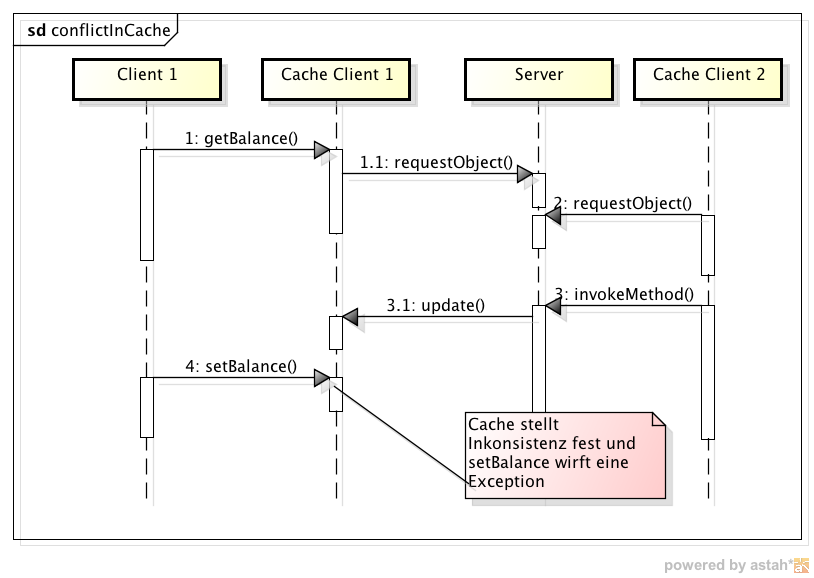
\includegraphics[scale=0.3]{images_objectcaching/conflictInCache}

Eine weitere Möglichkeit in welcher Reihenfolge Methodenaufrufe verarbeitet werden, beinhaltet dass der Server ein \verb|setBalance()|von einem Client erhält und bevor er das Update an alle versendet verarbeitet er ein \verb|setBalance() | eines anderen Clients. In diesem Fall detektiert der Server die Inkonsistenz. Beide Client haben sich die selbe Version des selben Objektes geholt.
\begin{enumerate}
\item Client 2 sendet ein \verb|setBalance()| an den Server. Bei der Verabeitung dieses Methodenaufrufs macht der Server drei Dinge in dieser Reihenfolge.
  \begin{enumerate}
  \item Methode auf Object ausführen
  \item Update an alle Clients senden
  \item Versionnummern der ConcurrencyControl für jeden Client updat\-en
\end{enumerate}
\item Client 1 sendet ebenfalls ein \verb|getBalance()|. Der Cache in Client 1 hat für den Methodenaufruf von Client 2 noch kein Update erhalten. Er wird an den Server weitergeleitet. Der Methodenaufruf trifft beim Server vor dem Versionsnummernupdate des Methodenaufrufs von Client 2 ein. Der Server stellt fest, dass Client 1 noch mit einer alten Version arbeitet und returniert Client 1 eine Exception.
\end{enumerate}

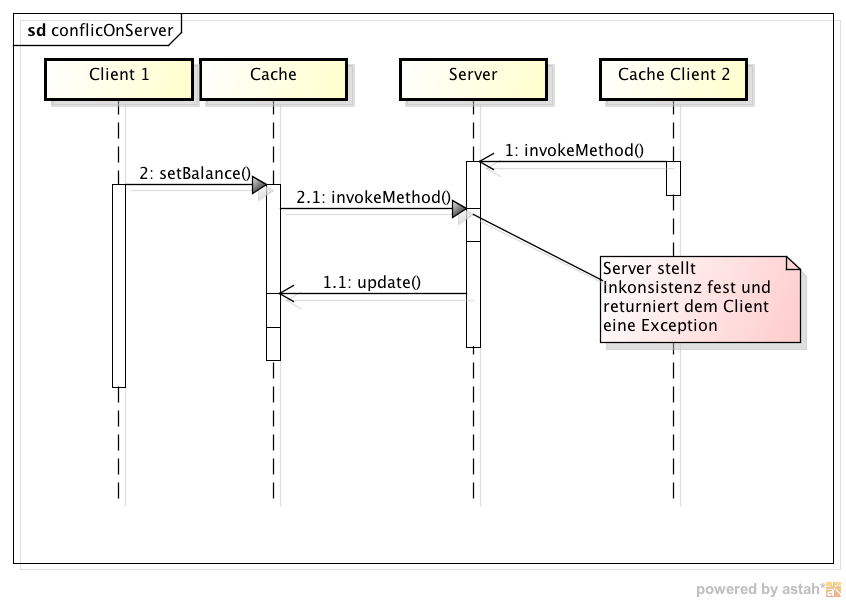
\includegraphics[scale=0.3]{images_objectcaching/conflictOnServer}

Bei allen Fällen kann Inkonsistenz festgestellt werden, indem sich der Server und der Clientcache merkt, welche Version an den Client vor dem \verb|setBalance()|herausgegeben wurde und überprüft, ob die Version des Objektes mittlerweile höher ist. Dabei müssen die Versionnummern im Cache und auf dem Server nicht synchron sein. Es gibt jedoch eine Aufrufabfolgemöglichkeit bei der Inkonsistenz entstehen kann, wenn man sich nur darauf verlässt, welche Versionsnummer zuletzt herausgegeben wurde.

\begin{enumerate}
\item Client 2 sendet ein \verb|setBalance()|. Der Server versendet das Update und aktualisiert die Versionsnummern der Clients.
\item Client 1 sendet ebenfalls ein \verb|setBalance()|. Er sendet den Methodenaufruf dem Server bevor er den Update erhalten hat. Zum Zeitpunkt der Ankunft des Methodenaufrufs beim Server, hat der Server aber bereits das Update versendet und die Versionsnummer aktualisiert. Der Methodenaufruf und der Update haben sich also gekreuzt. Da der Server meint, dass Client 1 mit der aktuellen Version arbeitet, wird er den \verb|setBalance()| Aufruf auf dem Objekt ausführen. Es kommt zu einem Lost Update.
\end{enumerate}

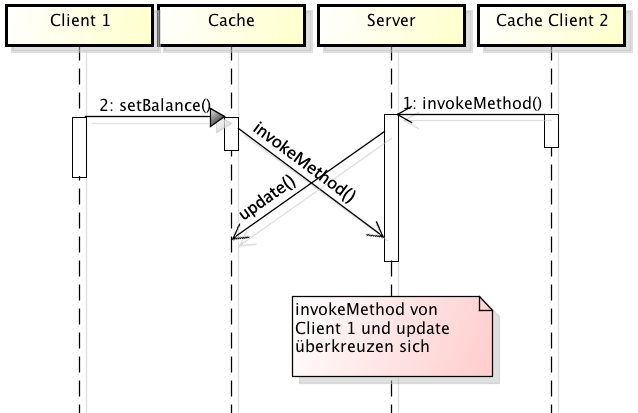
\includegraphics[scale=0.3]{images_objectcaching/conflictCross}

Um Inkonsistenz bei diesem Szenario zu erkennen und zu verhindern, muss die Nachricht die den \verb|setBalance()| Methodenaufruf enthält, die Versionnummer des Clients, der die Methode aufruft, mitsenden. Ist diese Versionnummer tiefer als die aktuelle Versionnummer des Objektes wird eine Exception geworfen. Damit die Versionnummern auf Server und auf Client immer synchron sind muss bei einem ObjectRequest die aktuelle Versionnummer an den Client gesendet werden. Bei einem Update wird die Nummer einfach inkrementiert.

\subsubsection{Erwartetet Vorteile}
\label{sec:erwartetet-vorteile}

\begin{itemize}
\item \verb+getBalance()+-Aufrufe werden schneller ausgeführt, da der Aufruf nicht über einen Socket geschickt werden muss, sondern im RAM bleibt, falls das Object im Cache vorhanden ist.
\item Bei \verb+setBalance()+ werden mögliche Inkonsistenzen bereits beim Client festgestellt. Der User erhält schneller Feedback und der Server wird weniger durch Concurrency Control belastet.
\end{itemize}

\subsubsection{Domain Klassen des Client}
\label{sec:domain-klassen}

\begin{description}
\item[Cache] Die Stubs, z.B. AccountStub, fordern beim Cache Objekte an. Der Cache holt die Objekte aus dem Memory oder er fodert sie über Netzwerk beim Server an. Er fordert sie beim Server an, wenn sie noch nicht vorhanden sind oder wenn ein Objekt invalidiert wurde. Der Cache muss bei einem Update, die Objekte im Hauptspeicher aktualisieren.
\item[Concurrency Control] Überprüft ob \verb+getBalance+ und \verb+setBalance()+ ausgeführt werden können, ohne dass Inkonsistenzen entstehen.

\item[Message Manager] Nimmt Messages für Remote-Methodenaufruf und Ob\-jekt\- -Request entgegen und sorgt dafür dass sie an den Server versendet werden und die Antwort darauf an den Absender weitergeleitet werden. Nimmt vom Server Update-Messages entgegen und leitet sie an den Cache weiter.

\end{description}

